\documentclass[11pt, a4paper]{article}

% --- Packages ---
\usepackage[utf8]{inputenc}
\usepackage[margin=1in]{geometry}
\usepackage{titlesec}
\usepackage{hyperref}
\usepackage{graphicx}
\usepackage{booktabs}
\usepackage{enumitem}
\usepackage{xcolor}
\usepackage{fancyhdr}

% --- Branding Colors ---
\definecolor{lightaccent}{RGB}{0, 120, 215}

% --- Header & Footer ---
\pagestyle{fancy}
\fancyhf{}
\lhead{\textbf{Technical Rider:} Somatic Sentience}
\rhead{Contact: +47 41275472 / gauteah@gmail.com}
\cfoot{\thepage}

% --- Document Info ---
\begin{document}

% --- Custom Title Page ---
\begin{titlepage}
    \centering
    
    % 1. Logo at the top
    
\includegraphics[width=0.3\textwidth]{../Figures/Black.png} \\ 
    \vspace{1cm}
    
    % 2. Title & Project Name
    %\hr
    \vspace{0.4cm}
    {\Huge \textbf{Technical Specification \& Rider}} \\
    \vspace{0.4cm}
    {\Large Project: Somatic Sentience} \\
    %\hr
    \vspace{1cm}
    
    % 3. Hero Photo of the Installation
    \begin{figure}[h]
        \centering
        \includegraphics[width=0.8\textwidth]{../Pictures/Kim x Tettpå 20 Feb 2026-237.png} % Your main installation photo
        \caption{\textit{Somatic Sentience in situ at Røverstaden}}
    \end{figure}
    
    \vspace{1cm}
    
    % 4. Author / Contact Details
    \vfill
    \textbf{Artist/Lead:} Gaute Holen / Naboklage \\
    \textbf{Contact:} gaute.ah@gmail.com | +47 41275472 \\
    %\textbf{Website:} [Your Website/Portfolio] \\
    \vspace{0.8cm}
    \large Last Updated: \today
\end{titlepage}

\thispagestyle{empty} % Ensures no headers on the title page
\newpage

\thispagestyle{empty}

\begin{abstract}
\noindent This document outlines the physical, electrical, and data requirements for the installation of \textbf{Somatic Sentience}. It is intended for site managers, production technicians, and safety officers.
\end{abstract}

\newpage
\tableofcontents
\newpage

% --- Section 1: Quick Specs Table ---
\section{Technical Summary (TL;DR)}
\begin{figure}[h]
    \centering
    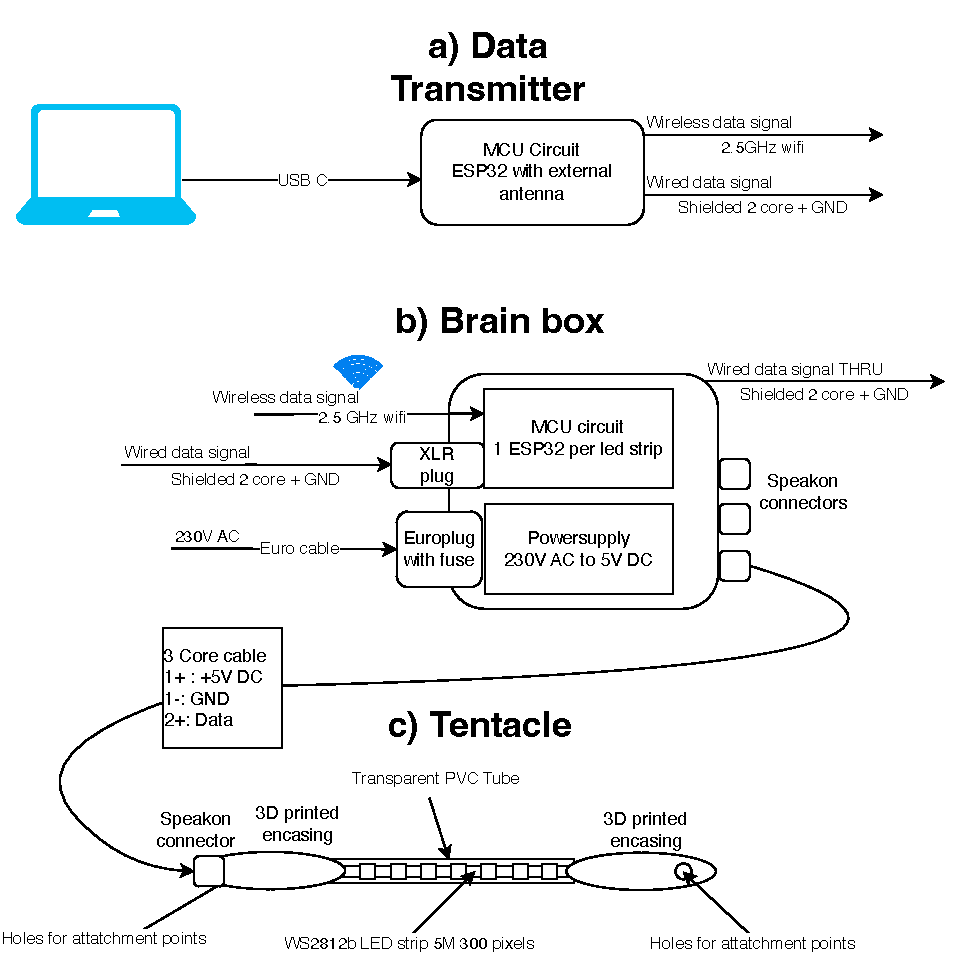
\includegraphics[width=0.8\textwidth]{../Figures/Diagram.pdf} % Your main installation photo
    \caption*{\textit{Fig 1: Somatic Sentience in situ at Røverstaden}}
\end{figure}


\begin{table}[h!]
\centering
\begin{tabular}{ll}
\toprule
\textbf{Parameter} & \textbf{Requirement} \\ \midrule
\textbf{Power Consumption} & [e.g., 1.2kW @ 230V] \\
\textbf{Footprint} & [e.g., 2m x 2m] \\
\textbf{Total Weight} & [e.g., 45kg] \\
\textbf{Signal Required} & [e.g., DMX512 / Art-Net / Standalone] \\
\textbf{Setup Time} & [e.g., 4 Hours] \\
\textbf{Rigging} & [e.g., 2x M10 Eye-bolts / Floor Standing] \\ \bottomrule
\end{tabular}
\end{table}

\section{Brain box}
\begin{figure}[h]
        \centering
        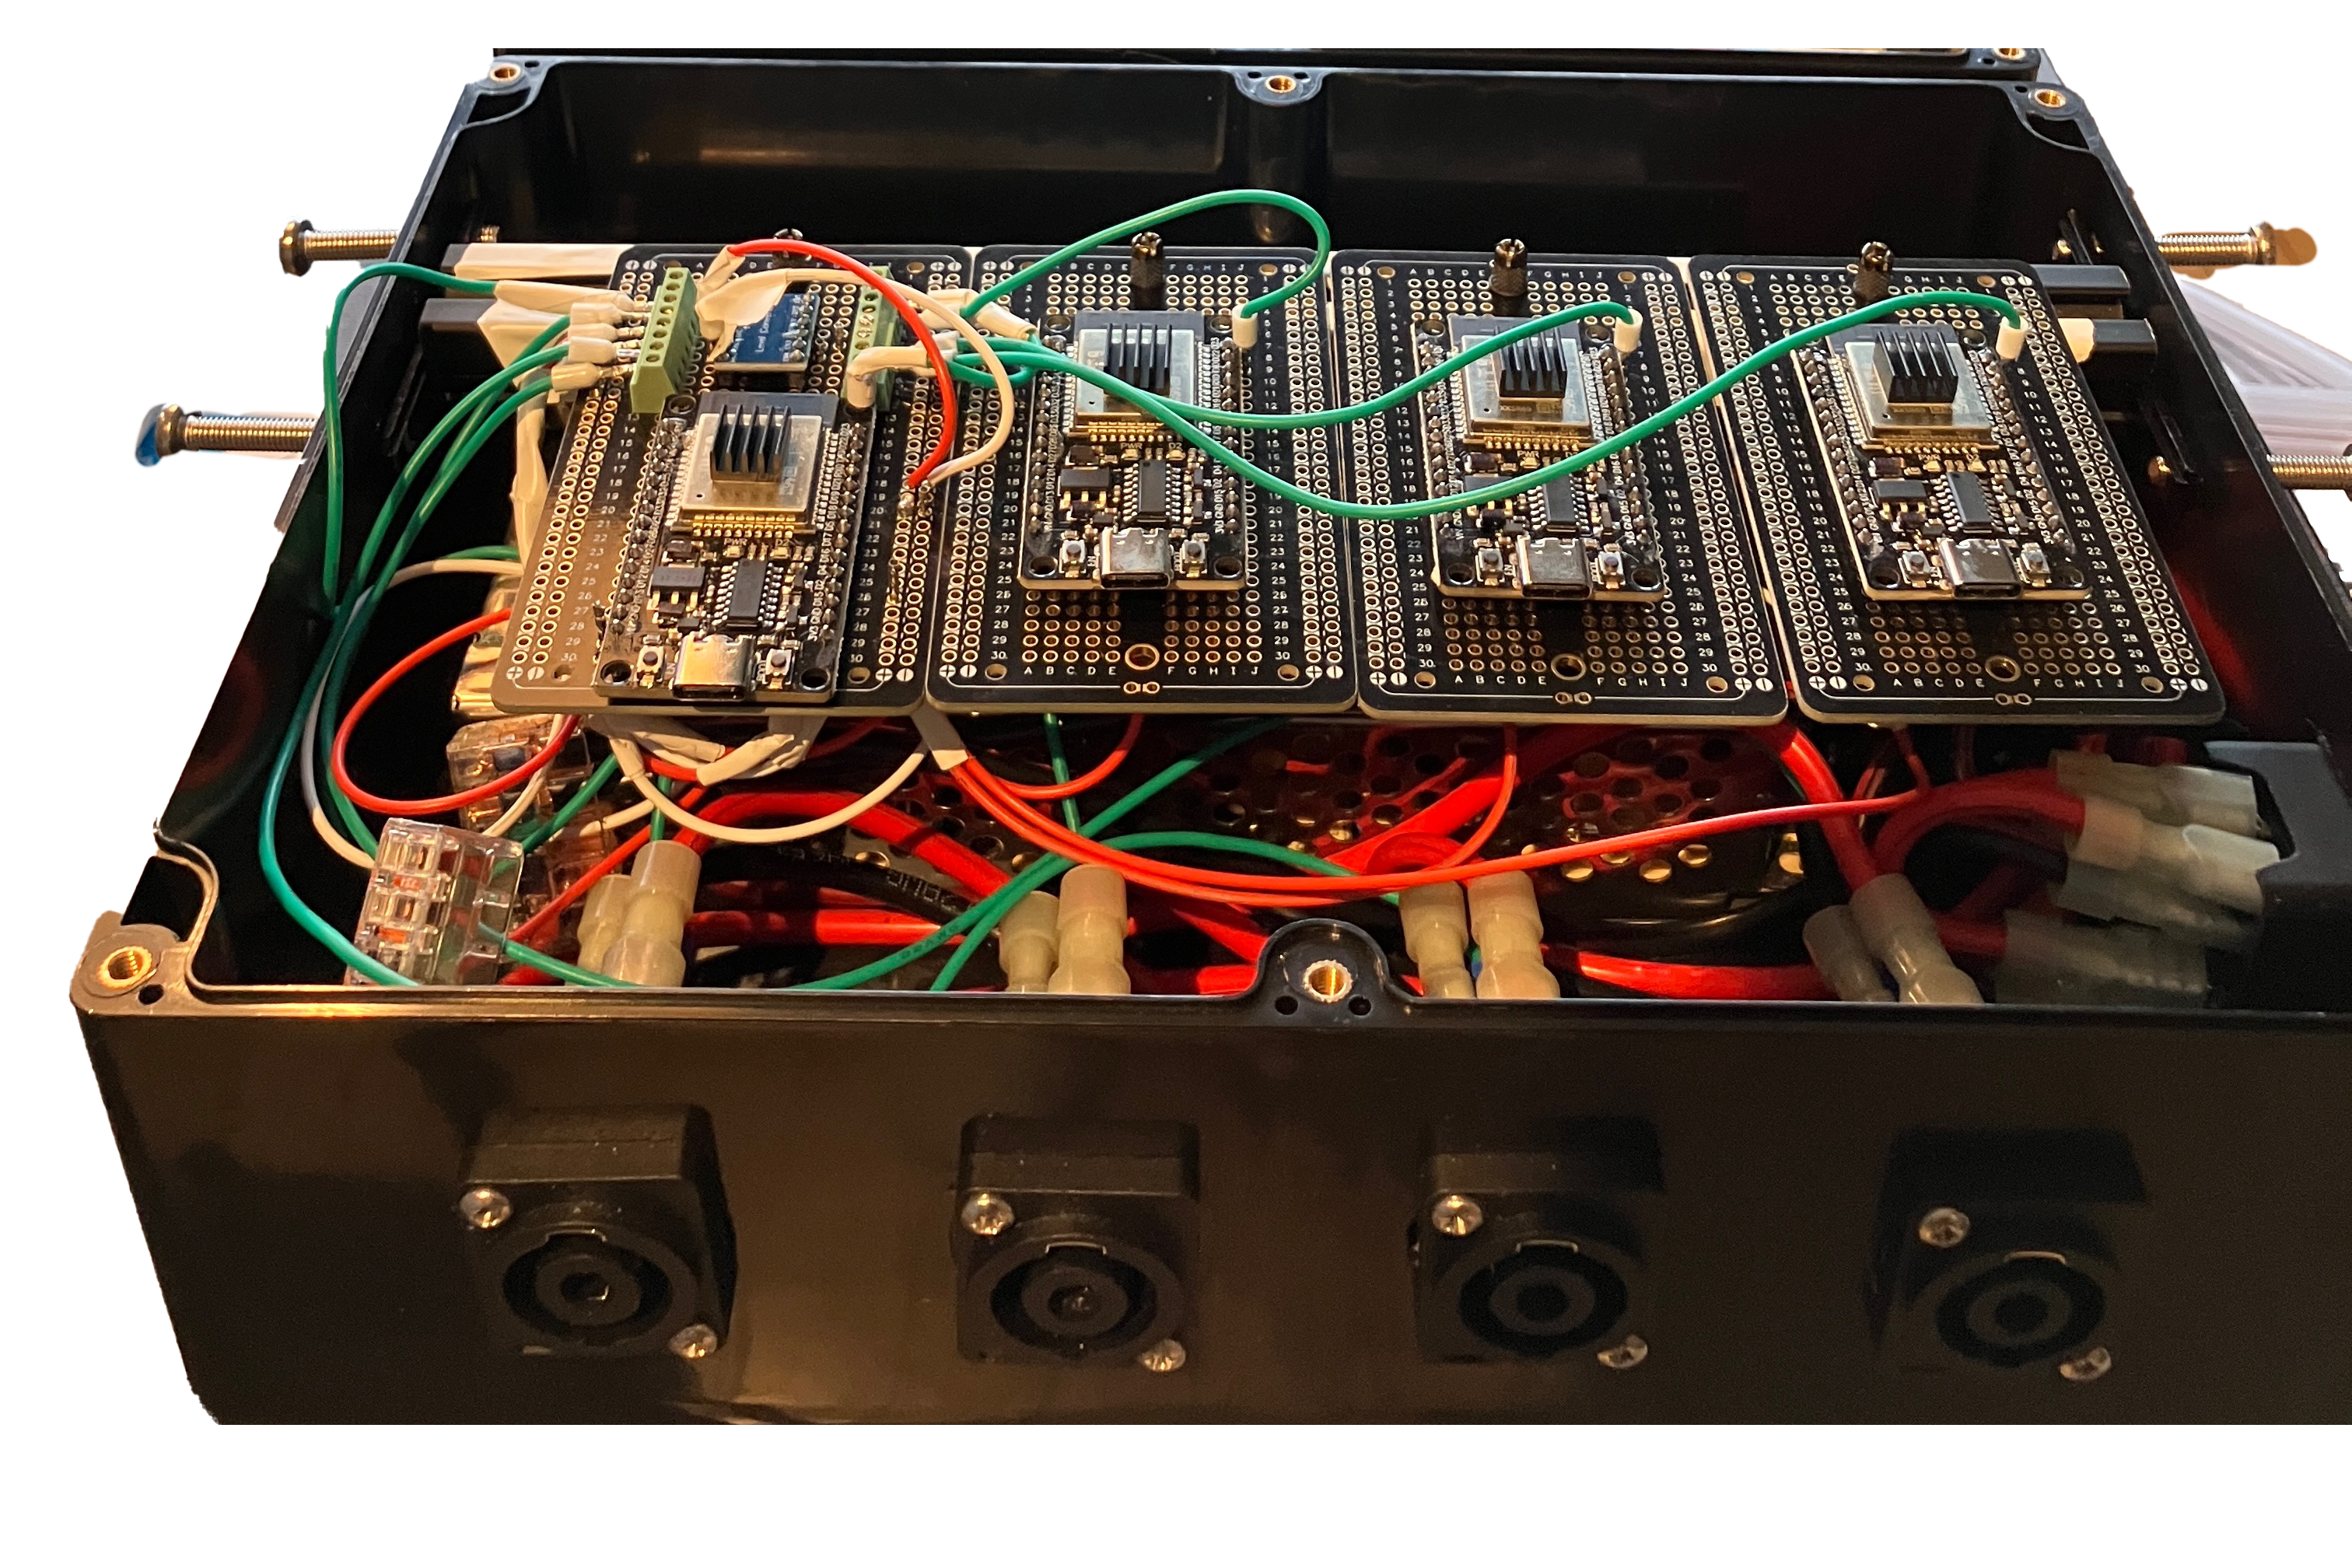
\includegraphics[width=0.8\textwidth]{../Figures/Brain.png} % Your main installation photo
        \caption{\textit{Somatic Sentience in situ at Røverstaden}}
    \end{figure}

\section{Tentacles}
\input{sec:tentacles.tex}

\section{Frames and mounting}
\input{sec:frames.tex}

% --- Section 2: Physical Requirements ---
\section{Physical \& Spatial Requirements}
\subsection{Dimensions \& Weight}
Detail the size when assembled. Include a "Clearance Zone" if the lights are moving or hot.
\begin{itemize}
    \item \textbf{Assembled Dimensions:} [W] x [D] x [H] cm.
    \item \textbf{Safety Perimeter:} [X] meters from the public.
    \item \textbf{Static Load:} [X] kg (Weight of the unit).
\end{itemize}

\subsection{Mounting \& Rigging}
How does it stay up? 
\begin{itemize}
    \item \textbf{Mounting Points:} [e.g., Standard 50mm truss clamps].
    \item \textbf{Safety:} [e.g., Secondary safety bond required at point X].
\end{itemize}

% --- Section 3: Electrical & Data ---
\section{Electrical \& Signal Specifications}
\subsection{Power Requirements}
\begin{itemize}
    \item \textbf{Connector Type:} [e.g., PowerCON, IEC, or Schuko].
    \item \textbf{Voltage:} [e.g., 110-240V AC, 50/60Hz].
    \item \textbf{Peak Current Draw:} [X] Amps.
\end{itemize}

\subsection{Signal \& Control}
How does the venue talk to your lights?
\begin{itemize}
    \item \textbf{Protocol:} [e.g., DMX512-A].
    \item \textbf{Channel Map:} [e.g., 12 Channels / Universe 1].
    \item \textbf{Connectivity:} [e.g., 5-pin XLR Male/Female].
\end{itemize}

% --- Section 4: Operation & Environment ---
\section{Operational Guidelines}
\subsection{Environmental Constraints}
\begin{itemize}
    \item \textbf{IP Rating:} [e.g., IP20 - Indoor use only].
    \item \textbf{Operating Temp:} [e.g., $10^\circ$C to $35^\circ$C].
    \item \textbf{Haze/Smoke:} [e.g., Compatible with water-based haze].
\end{itemize}

\subsection{Startup/Shutdown Procedure}
Briefly explain how the venue staff can turn it on/off safely.

% --- Section 5: Safety & Compliance ---
\section{Health \& Safety}
\begin{itemize}
    \item \textbf{Fire Safety:} [e.g., All materials treated with fire retardant NFPA 701].
    \item \textbf{Emergency Stop:} Location of the hard kill-switch.
\end{itemize}

\end{document}